	\section{Цель работы}
		Изучить базовые понятия нейротехнологий, ознакомиться с возможностями современных нейропакетов и получить навыки работы с ними.
	\section{Порядок выполенения работы}
		Дано 25 тыс. подписанных изображений кошек и собак. Данные взяты из соревнования Dogs vs Cats на сайте \href{https://www.kaggle.com/c/dogs-vs-cats}{Kaggle (https://www.kaggle.com/c/dogs-vs-cats)}.
			
		Разделим данные. 24500 изображений будут использованы для обучения и 500 для тестирования.
		
		В качестве сети используем свёрточную нейронную сеть. Свёрточная нейронная сеть (convolutional neural network, CNN) — специальная архитектура искусственных нейронных сетей, предложенная Яном Лекуном в 1988 году и нацеленная на эффективное распознавание изображений, входит в состав технологий глубинного обучения (англ. deep learning). Использует некоторые особенности зрительной коры, в которой были открыты так называемые простые клетки, реагирующие на прямые линии под разными углами, и сложные клетки, реакция которых связана с активацией определённого набора простых клеток. Таким образом, идея свёрточных нейронных сетей заключается в чередовании свёрточных слоев и субдискретизирующих слоев. Структура сети — однонаправленная (без обратных связей), принципиально многослойная. Для обучения используются стандартные методы, чаще всего метод обратного распространения ошибки. Функция активации нейронов (передаточная функция) — любая, по выбору исследователя.
			
		В качестве нейросетевого фреймворка используется TensorFlow.TensorFlow — открытая программная библиотека для машинного обучения, разработанная компанией Google для решения задач построения и тренировки нейронной сети с целью автоматического нахождения и классификации образов, достигая качества человеческого восприятия. TensorFlow применяются как для исследований, так и для разработки продуктов Google. TensorFlow является продолжением закрытого проекта DistBelief. Изначально, TensorFlow была разработана командой Google Brain для внутреннего использования в Google, а потом (9 ноября 2015 года) была переведена в свободный доступ с открытой лицензией Apache 2.0.
		
		Сверточный слой состоит из 32 фильтров и шагом = 5. Функция активации - ReLU. Сразу после этого добавляется максимальный уровень пула. Эта же конфигурация повторяется снова с 64 фильтрами. Также конфигурируются ещё слой с максимальным уровнем пула, 128 фильтров, затем снова 64 фильтра и 32 фильтра. Затем добавляется полностью подключенный слой с 1024 нейронами. Наконец, для завершения нашей модели используется отсеивающий слой с вероятностью 0,8. В качестве оптимизатора используется Adam с частотой обучения, равной 0,001. Функция потерь - это категориальная кросс-энтропия. Наконец, мы тренируем нашу сеть глубокого обучения в течение 10 эпох.
		\begin{ListingEnv}[H]
			\begin{Verb}
Training Step: 3829  | total loss: [1m[32m0.34434[0m[0m | time: 44.501s
| Adam | epoch: 010 | loss: 0.34434 - acc: 0.8466 -- iter: 24448/24500
Training Step: 3830  | total loss: [1m[32m0.35046[0m[0m | time: 45.619s
| Adam | epoch: 010 | loss: 0.35046 - acc: 0.8432 | val\_loss: 0.50006 - val\_acc:
0.7860 -- iter: 24500/24500 --
			\end{Verb}
			\caption{Вывод результата обучения}
			\label{list:hwplain}
		\end{ListingEnv}
		
		
		За 32 минуты сеть обучилась с точностью предсказания 85\%. Проверим качество результата на тестовой выборке:
		
	\begin{figure*}[h]
		\centering
		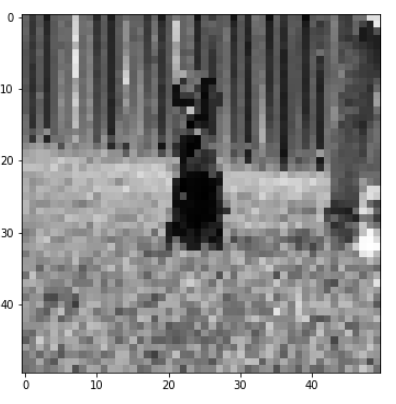
\includegraphics[width=0.7\linewidth]{god-as-cat}
		\caption{cat: 0.8773844838142395, dog: 0.12261549383401871}
		\label{fig:god-as-cat}
	\end{figure*}
	\begin{figure*}[h]
		\centering
		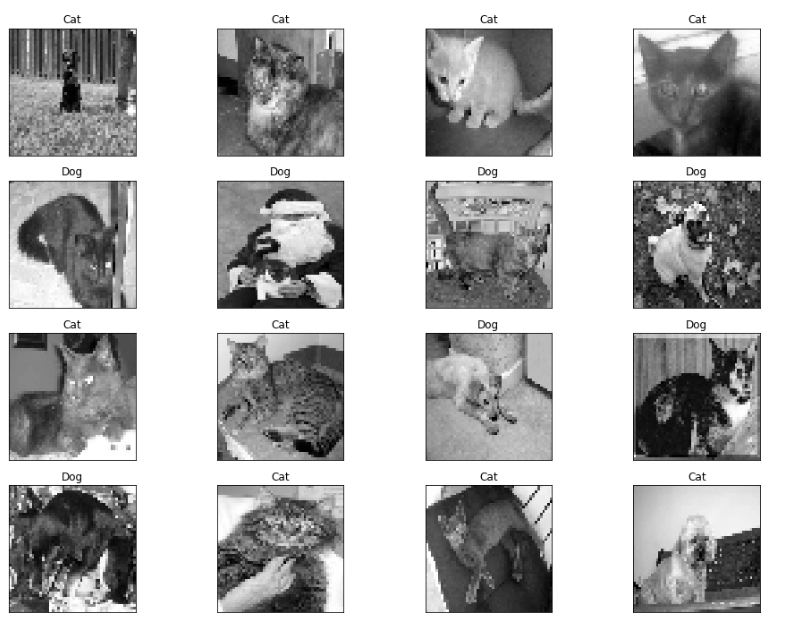
\includegraphics[width=1\linewidth]{images/cat-dog-result}
		\caption{Результат}
		\label{fig:cat-dog-result}
	\end{figure*}

	Как видно, сеть распознала деда мороза с котом на коленях как собаку. На тестовой выборке сеть показала 70\% точность, что значительно ниже результатов обучения.
	
	Используя данную архитектуру не удалось добиться лучших результатов за приемлемое время.

	\FloatBarrier
	\section{Вывод}
	Изучен фреймворк для построения нейронных сетей TensorFlow на примере решения типичной задачи классификации.
	Фреймворк гибкий и удобный, позволяет легко описывать нейронные сети сложных структур.
	Также за счёт использования графического процессора обучение происходит намного быстрее.
	Результат обучения нейронной сети не является выдающимся, однако учитывая то, что для распознавания использовались только пиксели изображения, приемлем.
	Для улучшения результата можно попробовать другую архитектуру, или изменить параметры оптимизатора.
	\newpage
	\section{Приложение}
	\lstinputlisting[caption={Программа на Python}, language=Python]{listings/cats-vs-dogs.py}